\subsection{Multilingual Distributed Representations without Word Alignment \cite{Hermann2013}}

This paper proposes a method for learning distributed representations in a multiligual setup. The model learns to assign similar embeddings to aligned sentences and dissimilar ones to sentences which are not aligned. It shows that the representations are semantically informative and applies them to a cross-lingual document classification task.

The basic idea is that, given enough parallel data, a shared representation would be forced to capture the common elements between sentences from different languages. What two parallel sentences have in common, of course, is the semantics of those two sentences. Using such parallel data, it proposes a novel method for learning vector representations at the word level and beyond.

The first step is to define a bilingual error function as follows: given a \emph{compositional sentence model (CVM)} $\mM_A$, which maps a sentence to a vector, it trains a second CVM $\mM_B$ using a parallel corpus $\mC_{A,B}$. For each pair of parallel sentences $(a,b) \in \mC_{A,B}$, it attempts to minimize
$$E_{dist}(a,b) = ||a_{root} - b_{root}||^2,$$
where $a_{root}$ ($b_{root}$) is the vector representing sentence $a$ ($b$).

The CVM used in this paper is a simple additive composition function:
$$a_{root}= \sum_{i=0}^{|a|} a_i.$$
Due to the use of parallel data, we know that $a$ and $b$ are semantically equivalent. Hence the goal is to jointly train both models $\mM_A$ and $\mM_B$, so that
$$E_{bi}(\mC_{A,B}) = \sum_{(a,b) \in \mC_{A,B}} E_{dist}(a,b)$$
is minimized.

However, the models could learn to reduce all embeddings and composition weights to zeros and thereby minimize the objective function. This problem is addressed by penalizing small distances between non-parallel sentence pairs. For every pair of parallel sentences $(a,b)$ it samples a number of additional sentences $n \in \mC_B$, which are not exact translation of $a$:
$$E_{noise}(a, b, n) = [1 + E_{dist}(a,b) - E_{dist}(a,n)]_{+},$$
where $[x]_{+} = \max(x,0)$ denotes the standard hinge loss. Thus, the final objective function is defined to be:
$$J(\theta_{bi}) = \sum_{(a,b) \in \mC_{A,B}} (\sum_{i=1}^k E_{noise}(a,b,n_i)) + \frac{\lambda}{2} || \theta_{bi} ||^2.$$

\begin{figure}[h]
  \centering
  % Requires \usepackage{graphicx}
  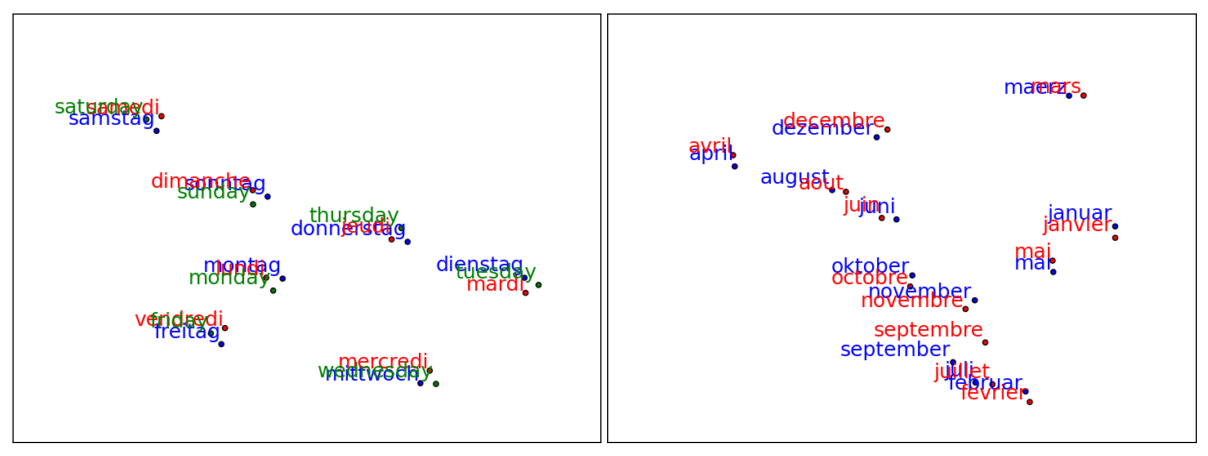
\includegraphics[width=\linewidth]{Hermann13-BiCVM.png}\\
  \caption{The left scatter plot shows t-SNE projections for a weekdays in three language. The right plots shows months using only the German and French words.}\label{fig:Hermann13-BiCVM}
\end{figure}

In the experimental study, the paper evaluates the proposed model in to experiments: the \emph{BiCVM} model was trained on 500k sentence pairs of a English-German parallel corpus. The \emph{BiCVM+} used this dataset in combination with anther 500k parallel sentences form the English-French section. The motivation behind BiCVM+ is to investigate whether it can learn better embeddings by introducing additional data in a different language. The models are evaluated on the \emph{cross-lingual document classification (CLDC)} task. It is shown that both models outperform all prior work on this task. Further, BiCVM+ outperforms BiCVM, indicating the usefulness of adding training data from a separate pair. Figure \ref{fig:Hermann13-BiCVM} shows the t-SNE projections for a number of English, French and German words.
